\chapter{Introdução}

% Falar da história
% processamento de imagens
%...

% Falar dos surveys

O trabalho foi baseado em dois Surveys
na área. O primeiro de Wei, Lefebvre, Kwatra
e Turk \cite{Wei2009} dá ênfase em
abordagens não paramétricas e texturas
dinâmicas. Já o segundo de Raad, Davy, 
Desolneux e Morel \cite{Raad2018} mostra
a síntese com métodos mais recentes
usando Deep Learning e Redes Convolucionais.
Analisando os dois Surveys, fica bem claro o 
quanto a área se modificou depois da
revolução do Deep Learning, que se iniciou
em 2015 com o trabalho de Yann LeCun, 
Yoshua Bengio e Geoffrey Hinton \cite{LeCun2015}.

\section{O que é textura}

% Falar do problema de definir textura
% - Na vida real
% - Em computação gráfica - imagem (conjunto de pixels)

% Definir textura como as características
% da superfície de um objeto

A palavra ``textura'' pode ter diferentes significados
dependendo do contexto.
Um deles se refere às
diferentes características da superfície de um objeto,
sejam elas visuais (cor, desenhos), geométricas (relevo,
forma) ou táteis (maciez, dureza). 
Em computação gráfica, textura geralmente é
o nome que se dá a uma imagem (matriz de pixels)
que descreve alguma
característica da superfície de um objeto,
como a cor ou a direção do vetor normal (utilizada
para iluminação).

% Restringir para texturas estacionárias
% representadas por imagens

Para o processo de síntese, é preciso restringir o
conjunto de imagens consideradas texturas àquelas
que apresentam algum tipo de padrão perceptual
em seu domínio. Com isso é possível fazer a síntese
estudando e imitando o processo que gerou esse padrão.

% Falar da definição com Markov Chain

Cross, G.R. e Jain, A.K. \cite{Cross1983} descrevem
textura como sendo um Campo Markiviano Aleatório
(Markov Random Field, MRF). Esse modelo é o mais
usado no processo de síntese pois satisfaz a propriedade
de Markov (o valor de cada pixel dado sua vizinhança não
depende do resto da textura) e a homogeneidade (a
distribuição é invariante por translação), logo
se encaixa com as necessidades descritas anteriormente.

\begin{figure}[!ht]
	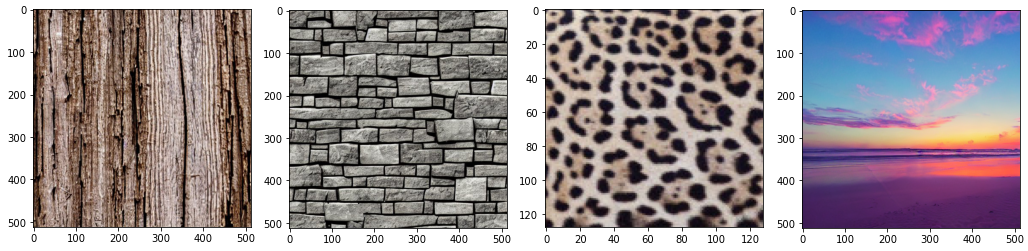
\includegraphics[width=\linewidth]{files/assets/texture.png}
	\caption{As três primeiras imagens são texturas por apresentarem
	um padrão visual estacionário. A quarta imagem apresenta
    uma estrutura não estacionária, não permitindo uma extrapolação
	infinita.}
	\label{img:preview}
\end{figure}

% Mostrar imagens de texturas

 

\section{O que é síntese de textura}

% Processo de gerar uma textura "nova"
% com mesma informação perceptual

O processo de síntese de textura baseado
em amostra não tem uma definição clara
matematicamente, é algo mais intrínseco
à percepção humana. O objetivo é,
a partir de uma amostra de textura,
gerar outras texturas de tamanho
arbitrário que imitam o processo
gerador da amostra. Esse processo
gerador é baseado em métricas
perceptuais, que não podem ser
definidas de forma fechada, pois
podem depender de aspectos
finos da imagem, como forma e 
iluminação.
Assim, os trabalhos na área
nos últimos anos consistem em
tentar descobrir melhores aproximações
para essa métrica perceptual.

% Inserir imagens de exemplo
\begin{figure}[!ht]
	\centering
	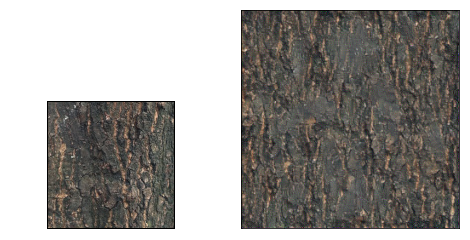
\includegraphics[width=\linewidth*2/3]{files/assets/sinth.png}
	\caption{Exemplo de síntese de textura. A imagem
	maior é visualmente semelhante a imagem menor.}
	\label{img:preview}
\end{figure}


% Pode ser interpretado como uma
% reamostragem da distribuição das texturas

Ao restringir o conjunto de imagens aos
Campos Markovianos, o processo de síntese
pode ser descrito como uma re-amostragem
da distribuição condicional da amostra.
Com isso, o desafio do método passa a ser 
descobrir a distribuição a partir
da amostra.


\chapter{Modelos}

Com o crescimento da área de processamento
de imagens e do poder computacional,
os modelos de Síntese de Textura foram
se aprimorando ao longo do tempo.
As melhorias são tando de qualidade
do resultado quanto no tempo de 
execução do método. Neste capítulo
será apresentado um breve resumo de
alguns dos principais modelos
da área.



\section{Modelos paramétricos}

Os modelos que fazem a síntese a partir
de um conjunto de estatísticas da amostra
original são chamados modelos paramétricos.
Esses modelos partem de um ruído e fazem
a síntese reduzindo
a diferença entre as estatísticas desse
ruído e da amostra utilizando uma função de 
otimização.
A qualidade do modelo vai depender do
conjunto de estatísticas escolhido
e do tipo de otimização utilizado.

% Heeger and Bergen [6] (matching histograms)

Heegen e Bergen \cite{Heeger1995} foram
um dos pioneiros no ramo. O método
parte de um ruído branco e faz a síntese
aproximando os histogramas das funções
de distribuição acumulada.
O método usa transformações
por pirâmides, que decompõe a imagem
em representações em diferentes escalas,
e faz a aproximação do histograma
em cada uma dessas camadas.
%Eles apresentam
%dois tipos de pirâmides, a Pirâmide 
%Laplaciana, que 
%e a Pirâmide Transladável (Steerable Pyramid)

\begin{figure}[!ht]
	\centering
	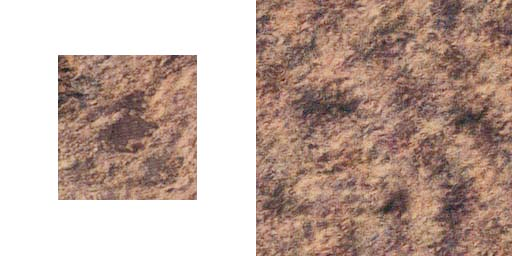
\includegraphics[width=\linewidth*2/3]{files/assets/articles/bergen.png}
	\caption{Síntese de Textura de Heegen e Bergen. O modelo
	conseguia sintetizar elementos estocásticos da textura.}
	\label{img:preview}
\end{figure}

% De Bonet [1] (multi-resolution)

De Bonet \cite{Bonet1997} propôs
um método que calcula a distribuição
conjunta da amostra em diferentes
escalas. Em seguida a amostragem
é feita partindo de escalas mais
grosseiras até escalas mais finas.

\begin{figure}[!ht]
	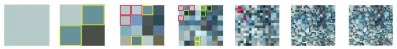
\includegraphics[width=\linewidth]{files/assets/articles/bonet2.png}
	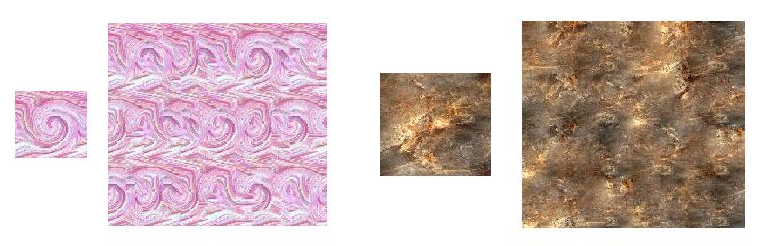
\includegraphics[width=\linewidth]{files/assets/articles/bonet.png}
	\caption{Modelo de De Bonet. O trabalho era feito escala
	por escala. Isso permitia sintetizar elementos mais regulares
    da textura.}
	\label{img:preview}
\end{figure}

% Zhu et al [12] (MRF - Gibbs sampling)
Zhu, Wu e Mumford \cite{Zhu1998}
utiliza um banco de filtros para
obter uma representação da imagem
e extrair o histograma.
Em seguida deriva-se a distribuição
desses filtros para serem re-amostrados
usando a técnica de Gibbs Sampling.

\begin{figure}[!ht]
	\centering
	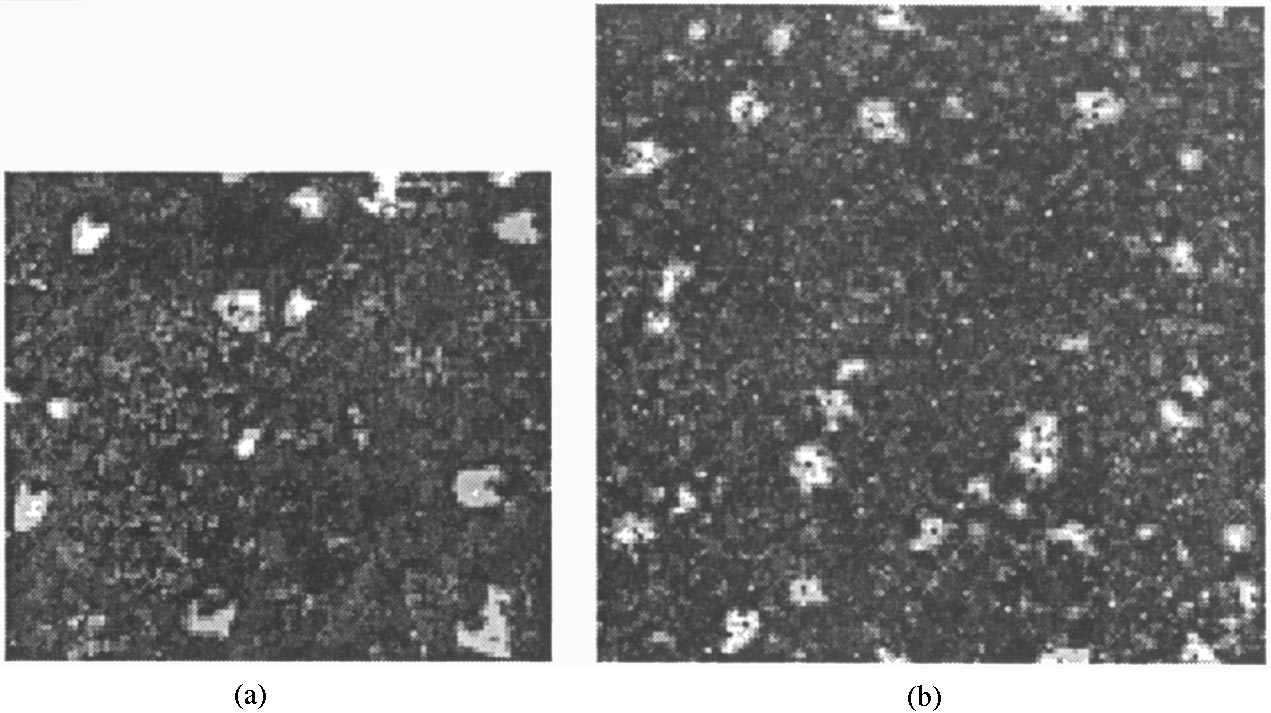
\includegraphics[width=\linewidth*2/3]{files/assets/articles/zhu.png}
	\caption{Modelo de Zhu, Wu e Mumford usando 5 filtros.}
	\label{img:preview}
\end{figure}


% Simoncelli and Portilla [9, 11] (wavelets)

Portilla e Simoncelli \cite{Portilla1999}
propuseram fazer a amostragem usando
as autocorrelações da Transformada
de Wavelet da amostra.

\begin{figure}[!ht]
	\centering
	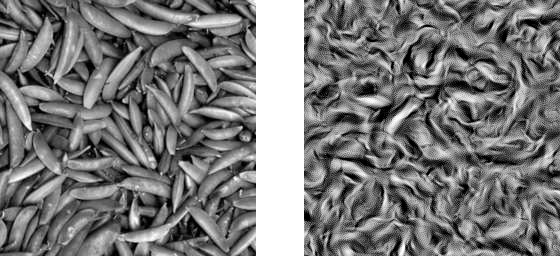
\includegraphics[width=\linewidth*2/3]{files/assets/articles/portilla.png}
	\caption{Teste do modelo de Portilla e Simoncelli com uma
	textura mais estruturado. É possível notar que há uma
	dificuldade em representar tais estruturas.}
	\label{img:preview}
\end{figure}


% Julesz’ hypothesis
% two images are perceptually equivalent if and 
% only if they agree on a set of statistic measurements.

% Falar da dificuldade em definir uma 
% estatística da informao perceptual

Béla Julesz foi um neurocientista que
trabalhava na percepção visual humana.
Em uma de suas publicações \cite{Julesz1981},
Julesz fez experimentos que mostravam
que um conjunto de imagens com mesma
informação visual podem ser representadas
pela densidade do que ele chama de
``Textons'', que são estruturas
como cor e arestas presentes na imagem.
Esse tipo de representação, embora tenha
guiado o trabalho de modelos paramétricos,
não deixa claro como fazer essa representação
em Textons. Assim, na tentativa de encontrar
tal representação, os métodos acabam sendo
difíceis de implementar, e nem sempre
conseguem ter sucesso em diferentes texturas.





\section{Modelos não paramétricos}

% Falar dos modelos que extraem informação
% diretamente da imagem

Diferentemente dos modelos paramétricos,
os modelos não paramétricos não dependem
do cálculo de alguma
estatística da amostra original para
o processo de síntese. Ele gera a imagem
pegando informação diretamente da
amostra de modo a simular a amostragem
da textura.

Essa forma de amostragem foi proposta
inicialmente por Efros e Leung \cite{Efros1999}.
Ela consistia em re-amostrar a textura
pixel por pixel, pegando diretamente
da imagem original o pixel que tem
a vizinhança mais parecida com a vizinhança
de seu destino. Os resultados na época
foram bem superiores aos que se podiam
obter com os métodos paramétricos,
mas a procura por todas as vizinhanças
na amostra tornava o método lento.

\begin{figure}[!ht]
	\centering
	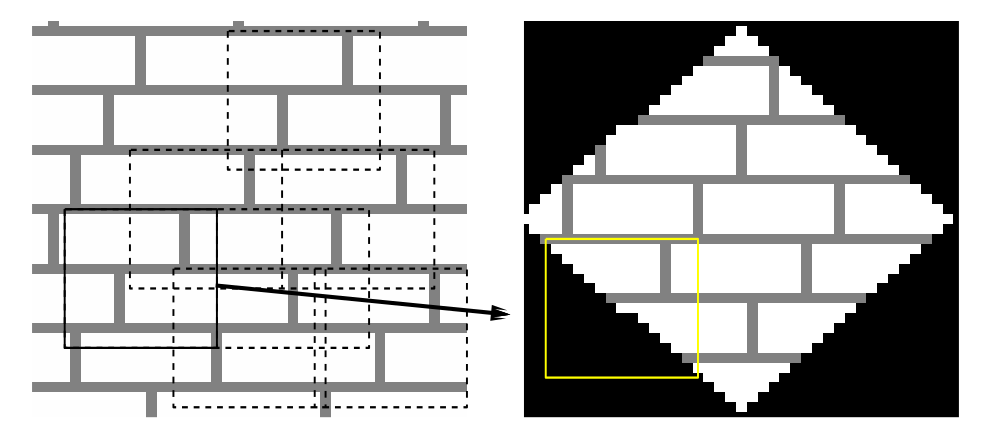
\includegraphics[width=\linewidth*2/3]{files/assets/articles/efros3.png}
	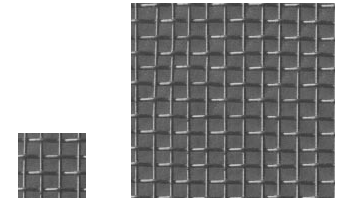
\includegraphics[width=\linewidth*5/6]{files/assets/articles/efros1.png}
	\caption{O algorítmo de Efros e Leung vai escolher o pixel
	com vizinhança mais parecida na amostra.}
	\label{img:preview}
\end{figure}

Mais tarde, Efros e Freeman \cite{Efros2001}
propuseram o método de Quilting (costura),
que fazia a amostragem a partir
de pedaços da imagem original. 
O método consistia em selecionar
janelas de tamanho fixo da amostra
e distribuí-las com uma sobreposição
sobre elas. Em seguida é usado
um algoritmo de min-cut para dividir
essas janelas em pedaços que se encaixam
para formar a nova textura.
Essa abordagem era mais rápida 
computacionalmente do que o método
anterior, e produzia resultados
tão bons quanto.

\begin{figure}[!ht]
	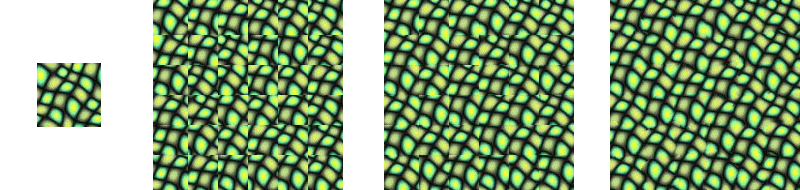
\includegraphics[width=\linewidth]{files/assets/articles/efros2.png}
	\caption{O modelo Quilting de Efros e Freeman escolhe pedaços
	aleatórios da amostra e encaixa os quadrados.}
	\label{img:preview}
\end{figure}

Com os avanços na área,
Vivek Kwatra \cite{Kwatra2005} propôs
uma amostragem fazendo a minimização
do que ele define como função de energia. 
Essa função é a diferença quadrática
entre as vizinhanças da textura gerada
e as vizinhanças mais próximas de cada uma.
O método usa uma variação do algoritmo EM, 
onde na faze ``E'' a energia é diminuída
por mínimos quadrados, e na faze ``M'' a
energia é diminuída escolhendo as
vizinhanças mais próximas na amostra.

\begin{figure}[!ht]
	\centering
	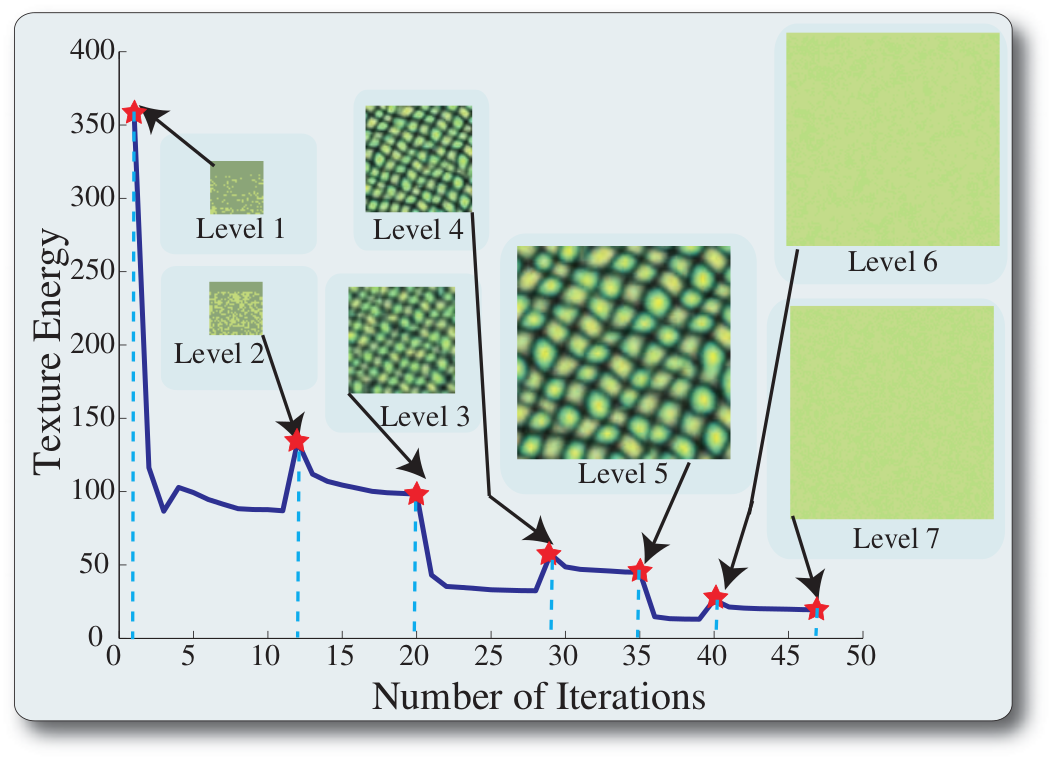
\includegraphics[width=\linewidth*2/3]{files/assets/articles/kwatra.png}
	\caption{Modelo de Vivek Kwatra. A função de energia 
	cai a cada nível de resolução.}
	\label{img:preview}
\end{figure}


\newpage
\section{Modelos de aprendizado profundo}

Os modelos de aprendizado profundo se aproveitam
dos avanços recentes que a área de Aprendizagem
de Máquina para melhorar o processo de síntese.
Os métodos a seguir utilizam as representações
geradas por redes treinadas para a detecção
de objetos para melhorar métodos paramétricos
de síntese já existentes.
As representações geradas por essas
redes conseguem sintetizar bem a informação
visual da imagem, oferecendo uma boa
métrica perceptual.

% Gatys

O primeiro a propor Síntese
de Textura baseado nesses modelos foram
Gatys, Ecker e Bethge \cite{Gatys2015}.
O trabalho utiliza as autocorrelações
da textura semelhante ao que foi proposto
por Portilla e Simoncelli, porém, em
vez de utilizar transformações da amostra
escolhidas a mão, utilizam a saída da
rede convolucional pré treinada. 
Esse método será tratado com detalhes
nesse trabalho, seguindo de uma implementação.

\begin{figure}[!ht]
	\centering
	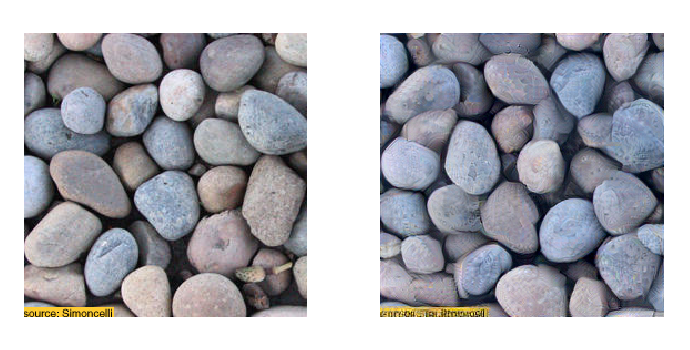
\includegraphics[width=\linewidth*2/3]{files/assets/articles/gatys1.png}
	\caption{Modelo de Gatys, Ecker e Bethge que
	utiliza as matrizes de Gram das convoluções.
	O método permite não fica muito preso na amostra
	e produz resultados mais criativos.}
	\label{img:preview}
\end{figure}

% Lu

Lu, Zhu e Wu \cite{Lu2016}
utilizam as representações
das redes convolucionais
no lugar do banco de filtros
no método de Zhu, Wu e Mumford,
produzindo melhores resultados sem
se preocupar com o tipo de filtros
escolhidos.

\begin{figure}[!ht]
	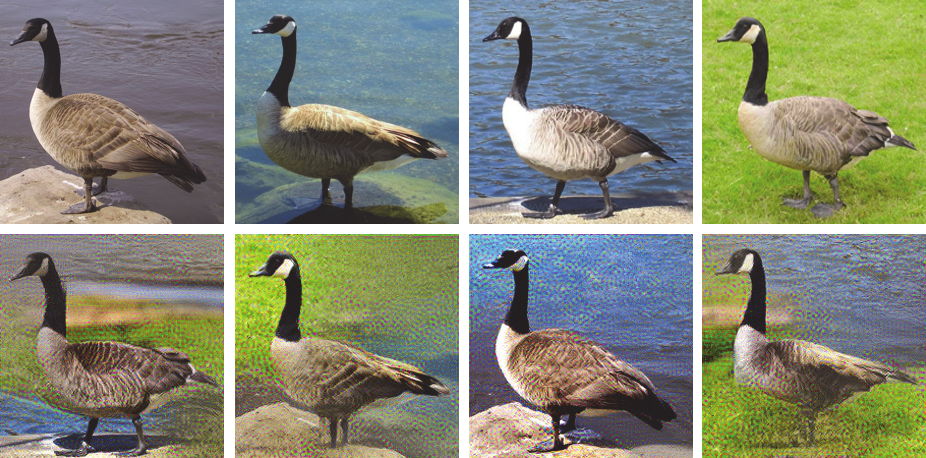
\includegraphics[width=\linewidth]{files/assets/articles/lu.png}
	\caption{Modelo de Lu, Zhu e Wu que pega quatro imagens como
	entrada (as de cima) e gera quatro imagens de saída (as de baixo).}
	\label{img:preview}
\end{figure}


% Falar de multiresolução? (De Bonet)

